\documentclass[10pt,a4paper,twocolumn]{report}  %紙張設定
\usepackage{xeCJK}%中文字體模組
\setCJKmainfont{標楷體} %設定中文字體
%\setCJKmainfont{MoeStandardKai.ttf}
\newfontfamily\sectionef{Times New Roman}%設定英文字體
%\newfontfamily\sectionef{Nimbus Roman}
\usepackage{enumerate}
\usepackage{amsmath,amssymb}%數學公式、符號
\usepackage{amsfonts} %數學簍空的英文字
\usepackage{graphicx, subfigure}%圖形
\usepackage{fontawesome5} %引用icon
\usepackage{type1cm} %調整字體絕對大小
\usepackage{textpos} %設定文字絕對位置
\usepackage{titlesec} %目錄標題設定模組
\usepackage{titletoc} %目錄內容設定模組
\usepackage{textcomp} %表格設定模組
\usepackage{multirow} %合併行
%\usepackage{multicol} %合併欄
\usepackage{CJK} %中文模組
\usepackage{CJKnumb} %中文數字模組
\usepackage{wallpaper} %浮水印
\usepackage{listings} %引用程式碼
\usepackage{hyperref} %引用url連結
\usepackage{setspace}
\usepackage{lscape}%設定橫式
%\lstset{language=Python, %設定語言
%		basicstyle=\fontsize{10pt}{2pt}\selectfont, %設定程式內文字體大小
%		frame=lines,	%設定程式框架為線
%}
\graphicspath{{./../images/}} %圖片預設讀取路徑
\usepackage{indentfirst} %設定開頭縮排模組
%\renewcommand{\figurename}{\Large 圖.} %更改圖片標題名稱
%\renewcommand{\tablename}{\Large 表.}
\renewcommand{\lstlistingname}{\Large 程式.} %設定程式標示名稱
\hoffset=-5mm %調整左右邊界
\voffset=-8mm %調整上下邊界
\setlength{\parindent}{2em}%設定首行行距縮排
\usepackage{appendix} %附錄
\usepackage{diagbox}%引用表格
\usepackage{multirow}%表格置中
%======== 版 面 設 定 ========%

\usepackage[top=3truecm,bottom=3truecm,
left=2truecm,right=2truecm]{geometry}
\setlength\columnsep{1cm}%調整雙欄位的中間間隔距離

\begin{document}
%=-------------------------內容----------------------=%
\begin{center}
\fontsize{11pt}{0}\sectionef
摘要
\end{center}
\begin{flushleft}
\qquad 本文目的是將實體機電系統簡化後導入虛擬環境並證明簡化後訓練的強化學習能算法能在虛擬環境中應用。

\qquad 將實體冰球機的機電系統簡化成一個自由度導入CoppeliaSim模擬環境透過Remote API控制環境中的冰球機移動,OpenCV來處理影像,強化學習訓練利用Open AI Gym的Pong Game測試參數。

\end{flushleft}
\begin{center}
\fontsize{10pt}{20pt}\selectfont 關鍵字: 類神經網路、強化學習、\sectionef CoppeliaSim、OpenAI Gym
\end{center}
%\chapter{前言}
\section{研究動機}
機器學習與各領域結合的應用越來越廣泛,在機電系統採用強化學習是為了讓機電系統的控制達到最佳化。本專題以實體的冰球機(圖.\ref{fig.冰球機})之機電系統作為訓練模型,將實體機器轉移到虛擬環境(圖.\ref{fig.模擬冰球機})進行模擬,為了找到適合的演算方式,因此將模型簡化(圖.\ref{fig.pong_gym})後再進行測試各種算法的優劣,透過不斷的訓練來得到一個優化過的對打系統。\\
\iffalse
\begin{figure}[hbt!]
\begin{center}
\subfigure{
\begin{minipage}[t]{0.3\linewidth}  %設定圖片間距
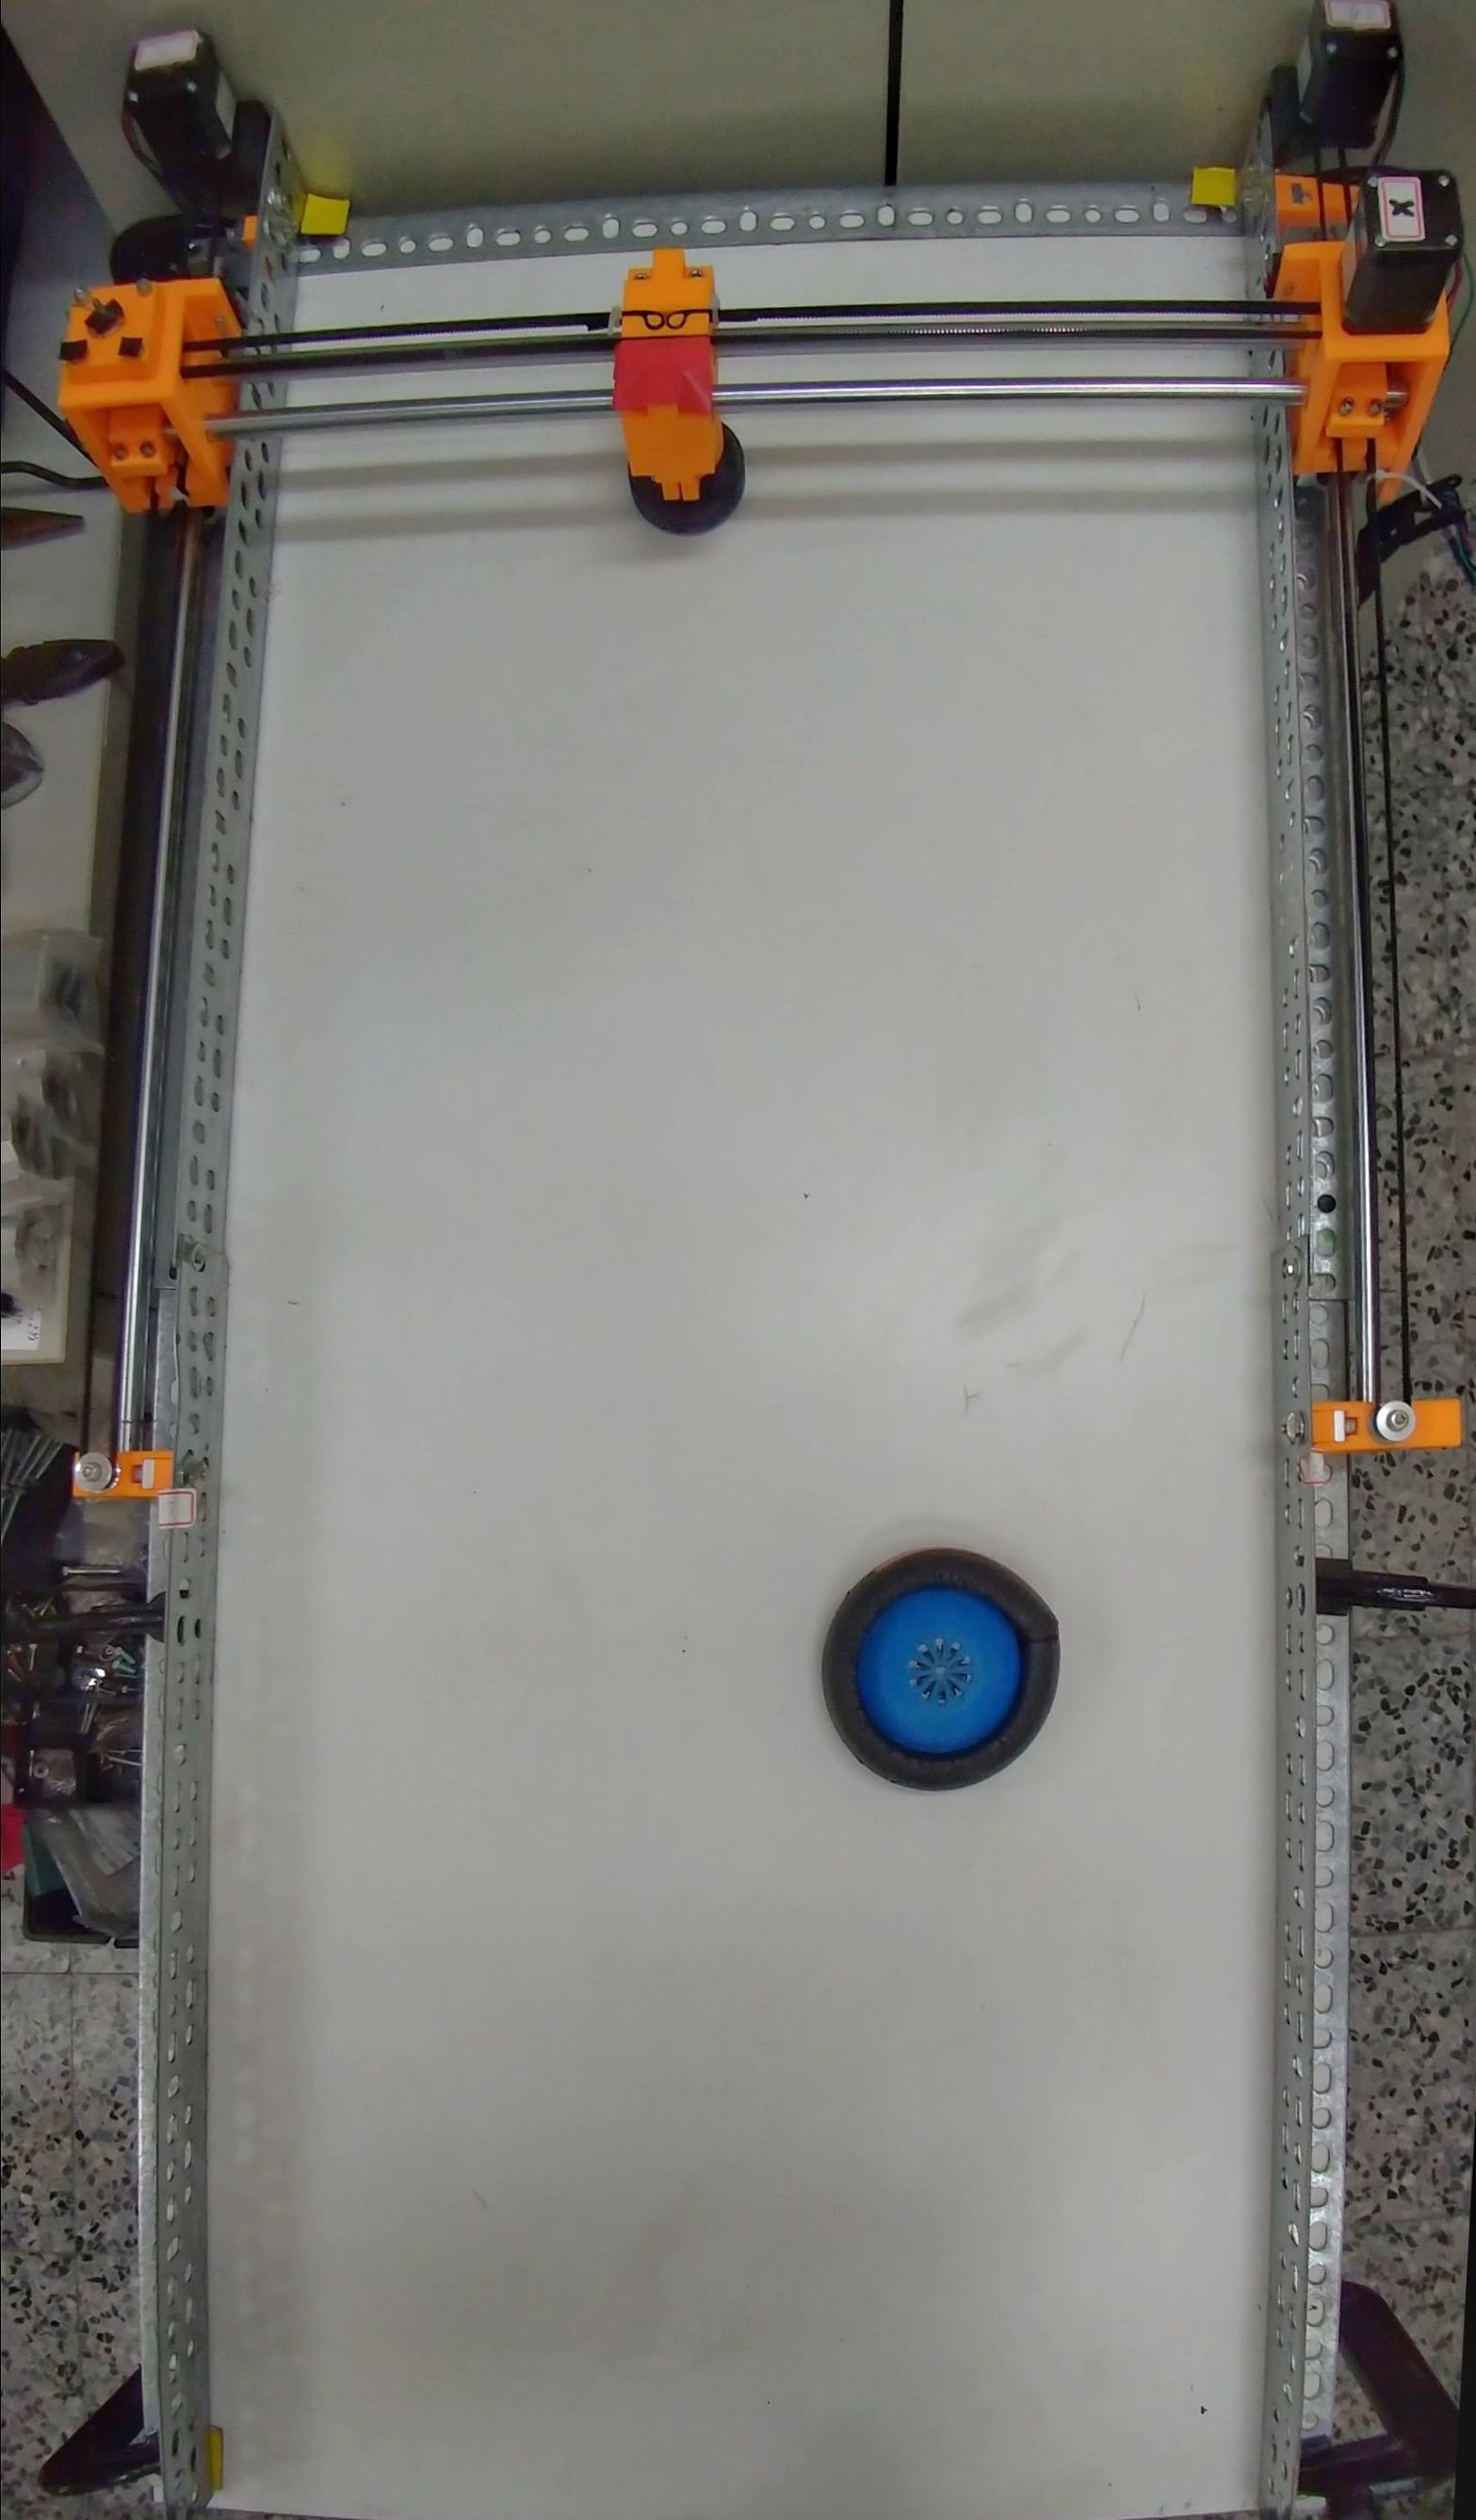
\includegraphics[width=4cm]{冰球機}
\caption{\Large 實體的冰球機}\label{fig.冰球機}
\end{minipage}
}
\subfigure{
\begin{minipage}[t]{0.3\linewidth}
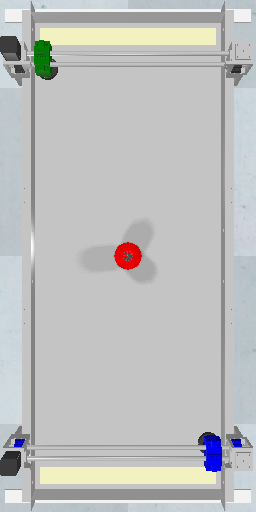
\includegraphics[width=4cm]{origin}
\caption{\Large 虛擬環境簡化後的冰球機}\label{fig.模擬冰球機}
\end{minipage}
}
\subfigure{
\begin{minipage}[t]{0.3\linewidth} 

\includegraphics[width=4cm]{pong_gym}
\caption{\Large Gym的Pong game}\label{fig.pong_gym}
\end{minipage}
}
\end{center}
\end{figure}
\fi
\section{研究目的與方法}
 本研究分三大部分,第一運用OpenAI Gym裡內建編譯的ATARI 2600遊戲Pong-v0,來作為訓練環境,加上強化學習的理論,測試不同演算法以訓練出最佳化的對打系統,第二換為CoppilaSim模擬環境並套用訓練程式,成為優化的對打機電系統。第三則是透過架設伺服器與虛擬環境結合。\\
 
 利用Gym的訓練環境來測試不同的算法所得到的訓練結果,比較不同算法、參數間的差異,並找出較適合Pong game的算法、參數,循序漸進提高環境的真實程度,來減少一開始就是以實體的方式測試所帶來硬體、程式、時間和金錢等成本。\\

 將Gym的訓練環境轉換到CoppilaSim模擬環境,利用貼近真實的模擬環境來修正在純程式的架構(Gym)與真實環境間的誤差,雖然CoppilaSim模擬環境與真實環境仍有些微的落差,兩者相比CoppilaSim的環境已非常貼近真實了,拉近了虛擬與現實間的距離,提高了實用性的價值。這部分還有利用OpenCV進行影像處理並撰寫輔助對打程式來協助玩家預判球的移動路徑或彈射位置。影像處理除了應用在輔助對打上,最主要是應用在訓練強化學習所需的輸入訓練影像。\\
 
 再透過架設伺服器與虛擬環境結合:讓虛擬環境的影像透過網伺服器串流影像供使用者遠端進行操控虛擬環境的擊錘進行打球,或是提供多人進行觀看對打影像。
\iffalse
\begin{figure}[hbt!]
\begin{center}
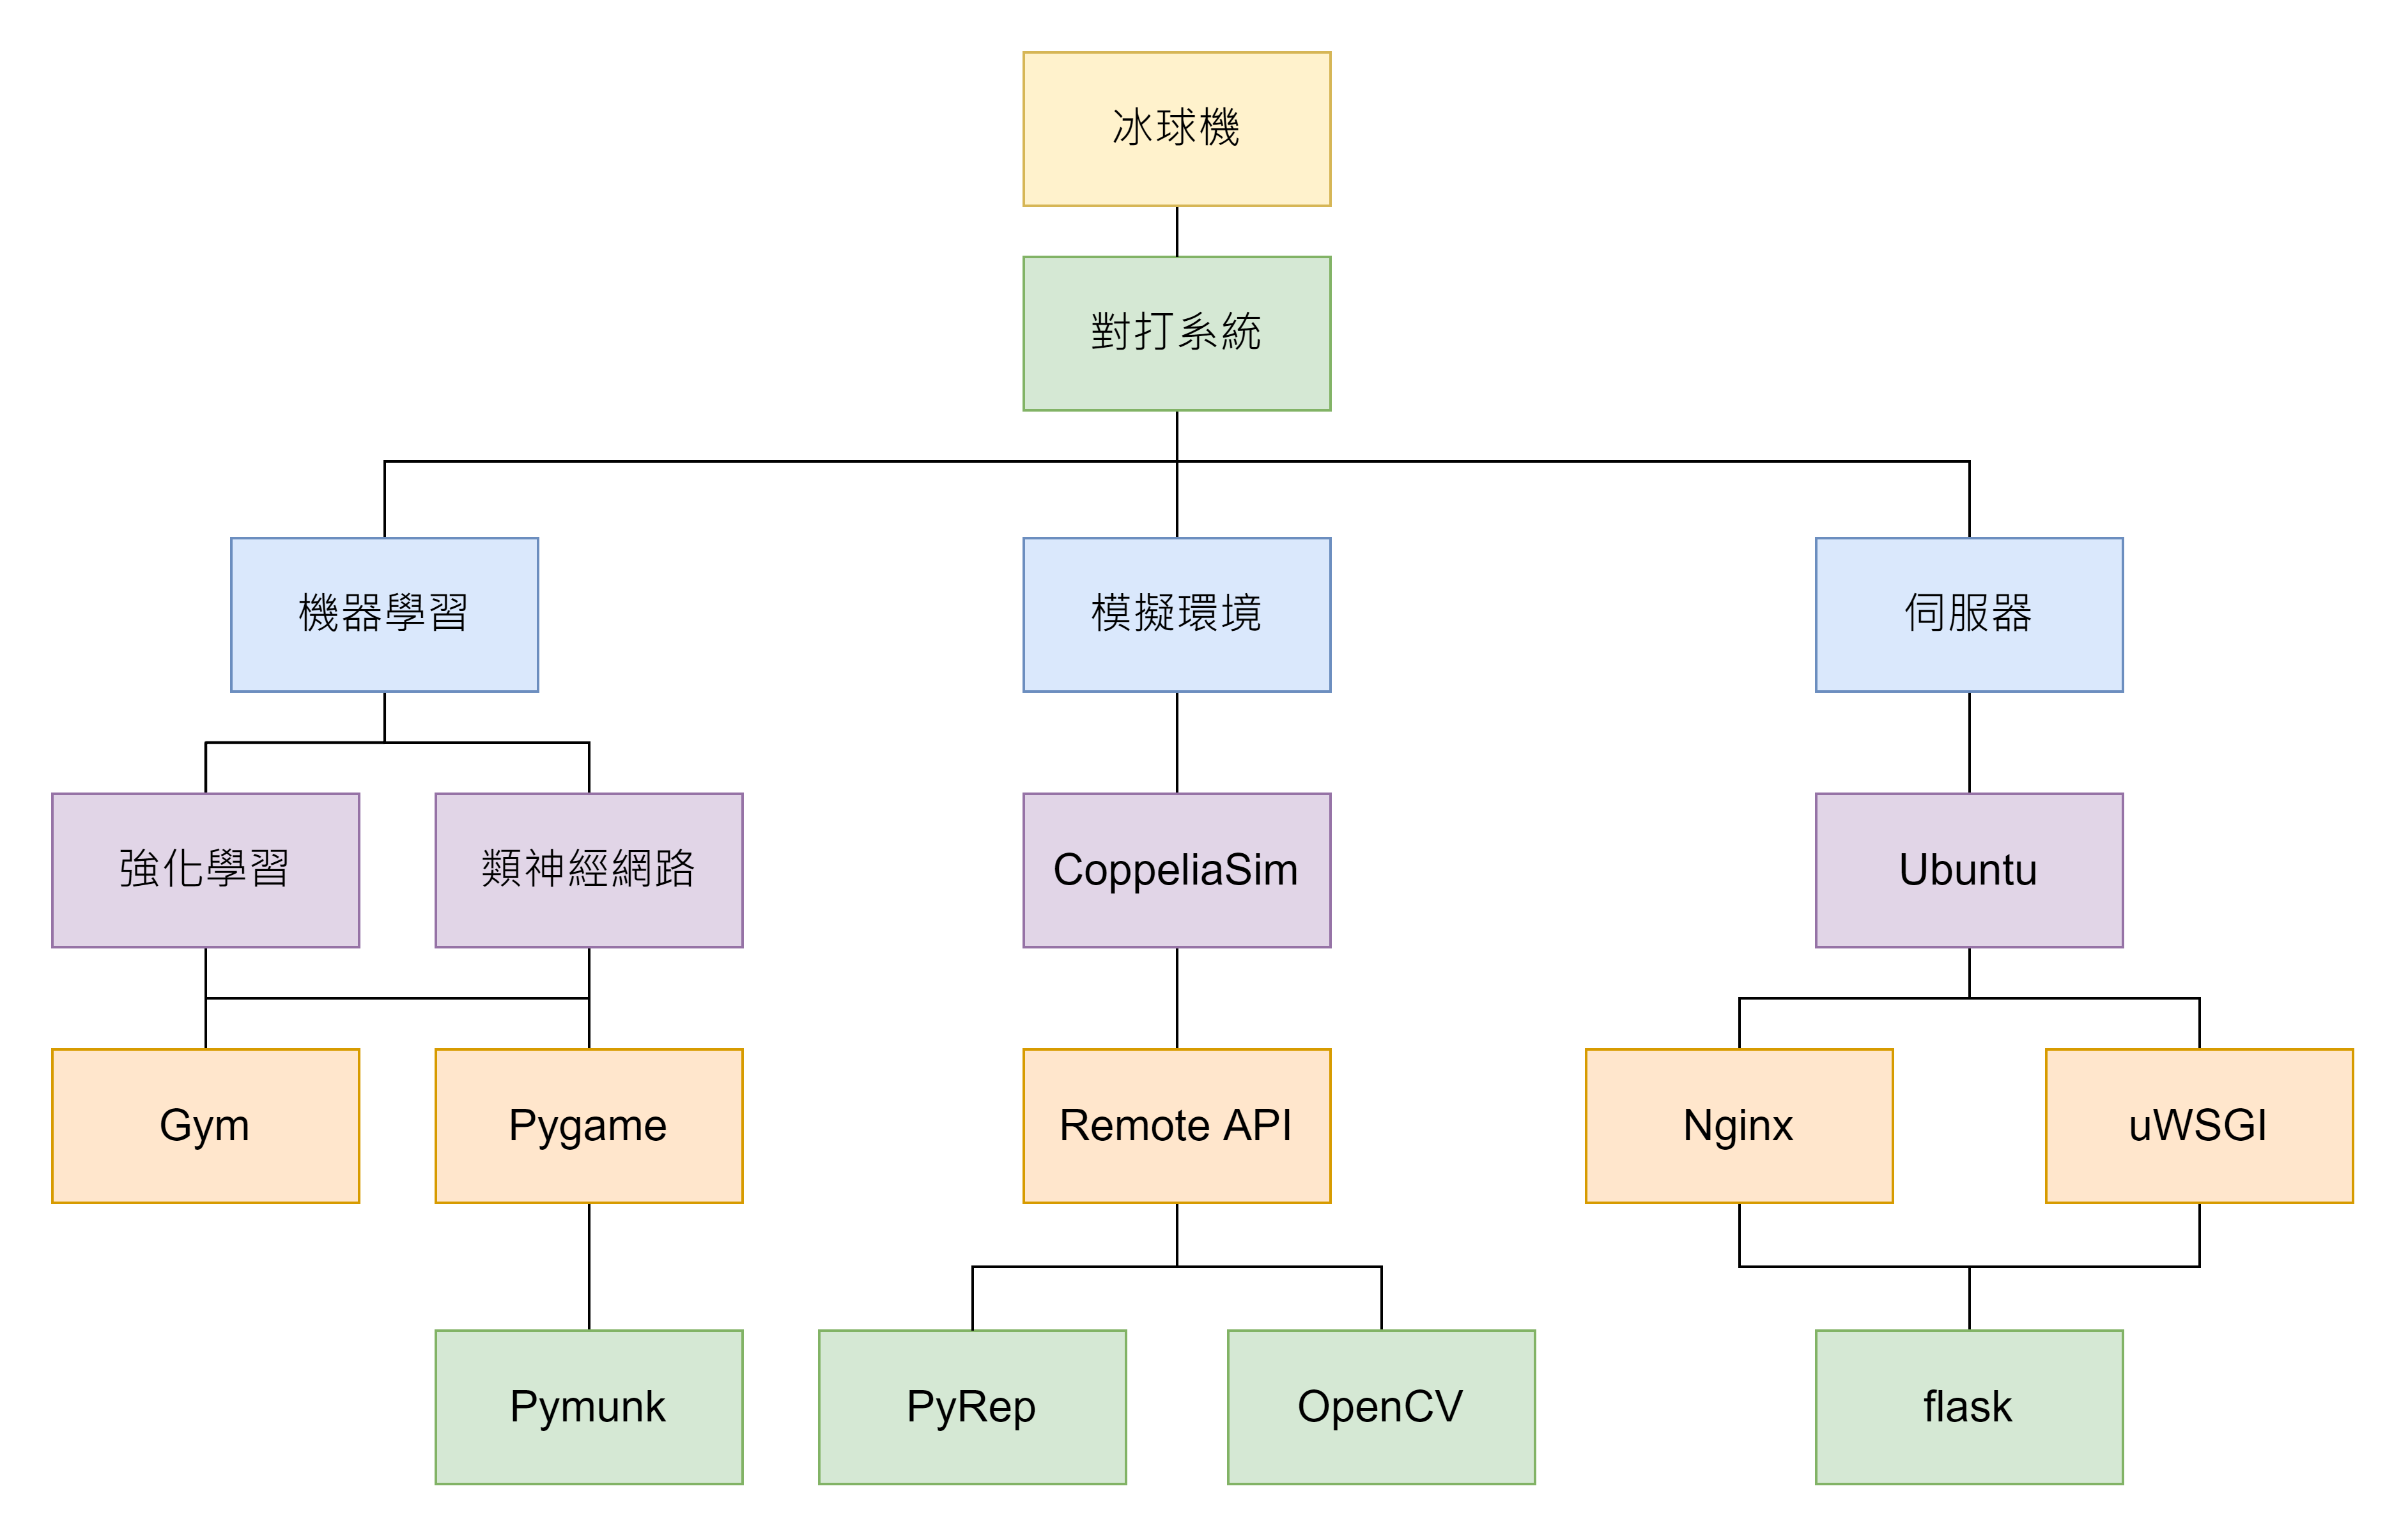
\includegraphics[width=15cm]{研究架構}
\caption{\Large 研究架構 }
\label{研究架構 }
\end{center}
\end{figure}
\fi
\section{未來展望}
此專題希望能利用現有完成的機械學習的算法,能發展成虛擬訓練,再將訓練完的機器學習應用到虛擬環境或是實體機電系統,並透過伺服器將影像串流提供玩家網頁介面進行遠端操控,同時提供多人觀看及時的比賽影像,將整個冰球機的控制和使用者間有更完善串聯,機電系統的部分達到最優化控制和虛實整合的應用。

\chapter{Literature Review}
Atari Video Computer System 是Atari Inc在1977年9月11日發行的一款家用遊戲機,直到1982年更名為Atari 2600,Pong是第一個主要發行的遊戲。OpenAI是一個人工智慧研究實驗室,研究著重於強化學習,Gym 具有多種不同的環境,並以標準化定義環境,其中包括Atari 2600的遊戲、Classic control、Box2D等環境供機器學習訓練使用。\\

\qquad Pong是一個2D的運動遊戲,模擬乒乓球對打,透過影像識別擊錘及球的位置訓練一個
\chapter{設計流程}
\section{研究動機}
機器學習與各領域結合的應用越來越廣泛,在機電系統採用強化學習是為了讓機電系統的控制達到最佳化。本專題以實體的冰球機(圖.\ref{fig.冰球機})之機電系統作為訓練模型,將實體機器轉移到虛擬環境(圖.\ref{fig.模擬冰球機})進行模擬,為了找到適合的演算方式,因此將模型簡化(圖.\ref{fig.pong_gym})後再進行測試各種算法的優劣,透過不斷的訓練來得到一個優化過的對打系統。\\

\section{研究目的與方法}
 本研究分三大部分,第一運用OpenAI Gym裡內建編譯的ATARI 2600遊戲Pong-v0,來作為訓練環境,加上強化學習的理論,測試不同演算法以訓練出最佳化的對打系統,第二換為CoppilaSim模擬環境並套用訓練程式,成為優化的對打機電系統。第三則是透過架設伺服器與虛擬環境結合。\\
 
 利用Gym的訓練環境來測試不同的算法所得到的訓練結果,比較不同算法、參數間的差異,並找出較適合Pong game的算法、參數,循序漸進提高環境的真實程度,來減少一開始就是以實體的方式測試所帶來硬體、程式、時間和金錢等成本。\\

 將Gym的訓練環境轉換到CoppilaSim模擬環境,利用貼近真實的模擬環境來修正在純程式的架構(Gym)與真實環境間的誤差,雖然CoppilaSim模擬環境與真實環境仍有些微的落差,兩者相比CoppilaSim的環境已非常貼近真實了,拉近了虛擬與現實間的距離,提高了實用性的價值。這部分還有利用OpenCV進行影像處理並撰寫輔助對打程式來協助玩家預判球的移動路徑或彈射位置。影像處理除了應用在輔助對打上,最主要是應用在訓練強化學習所需的輸入訓練影像。\\
 
 再透過架設伺服器與虛擬環境結合:讓虛擬環境的影像透過網伺服器串流影像供使用者遠端進行操控虛擬環境的擊錘進行打球,或是提供多人進行觀看對打影像。
 \iffalse
\begin{figure}[hbt!]
\begin{center}
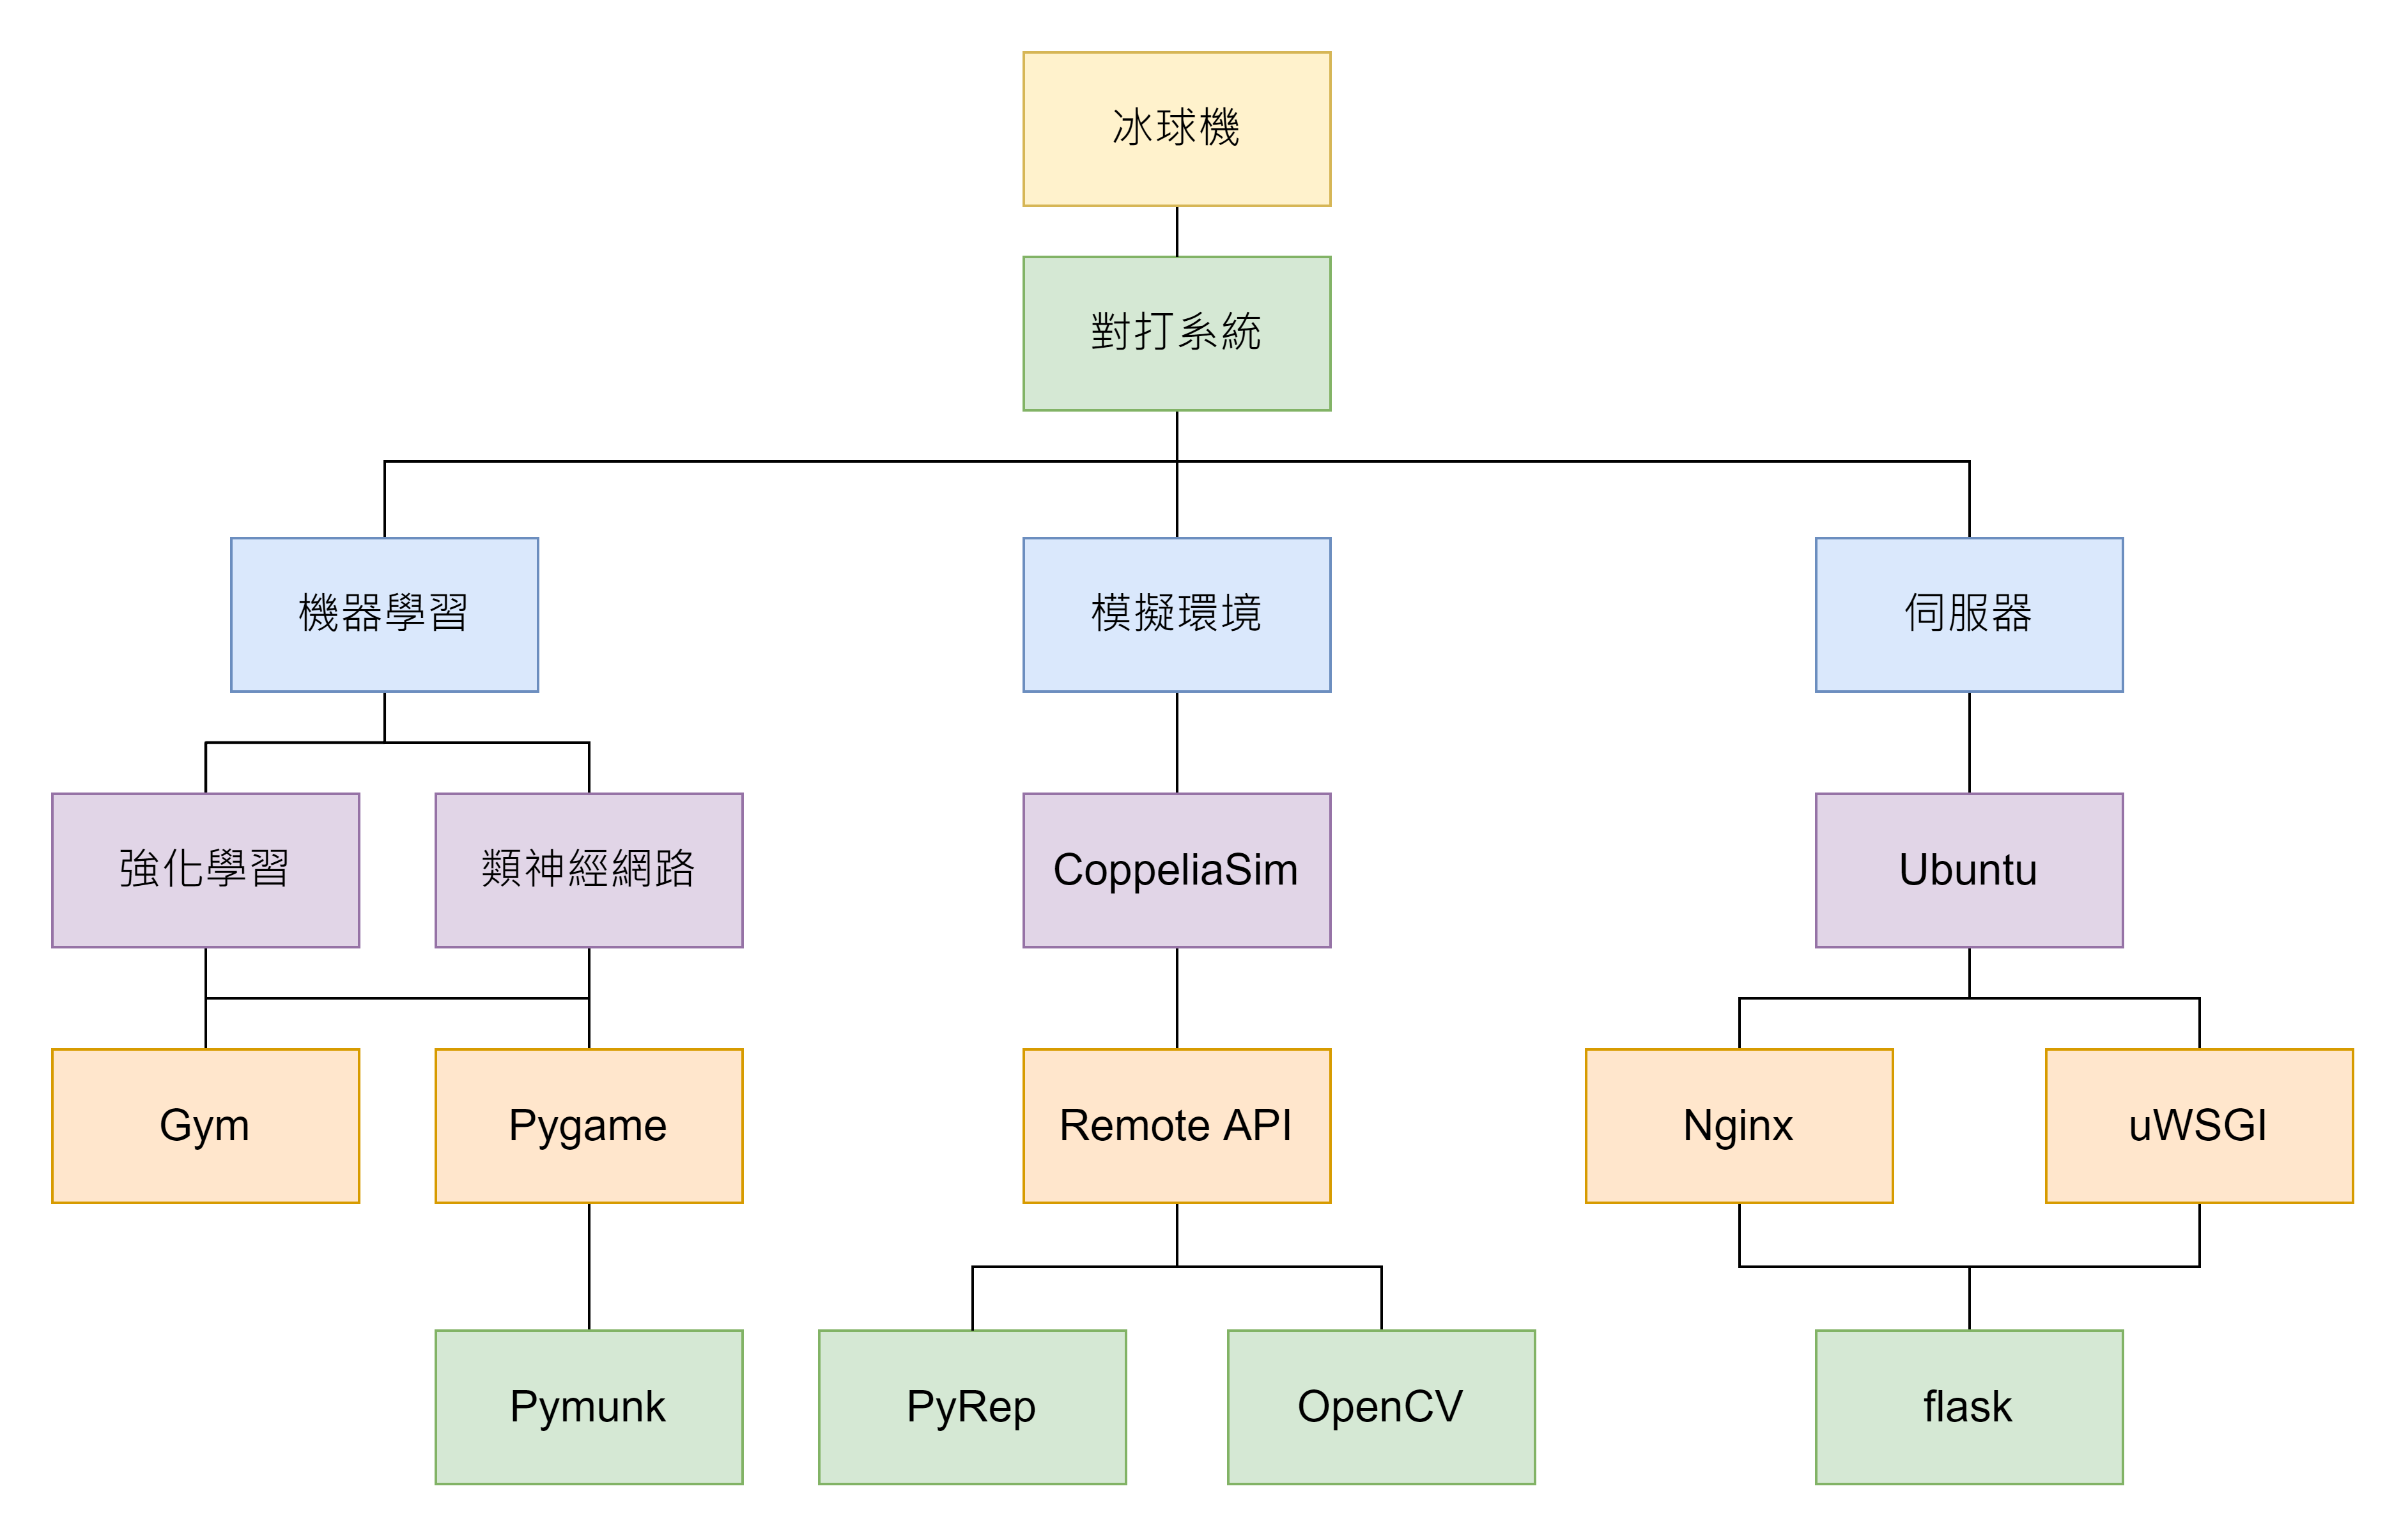
\includegraphics[width=15cm]{研究架構}
\caption{\Large 研究架構 }
\label{研究架構 }
\end{center}
\end{figure}
\fi

\section{未來展望}
此專題希望能利用現有完成的機械學習的算法,能發展成虛擬訓練,再將訓練完的機器學習應用到虛擬環境或是實體機電系統,並透過伺服器將影像串流提供玩家網頁介面進行遠端操控,同時提供多人觀看及時的比賽影像,將整個冰球機的控制和使用者間有更完善串聯,機電系統的部分達到最優化控制和虛實整合的應用。

\end{document}